\chapter{实现细节}
\label{chap:implements}
前一章中,我们已经介绍了整个系统的架构设计,这一章我们会对系统各个模块的一些实现细节进行详细阐述,主要涉及到方案选取、环境部署、算法设计与实现、系统性能调优等。一方面是对整体架构设计的补充论述,另一方面,我们会更多的讨论在实现过程中遇到的各种问题,以及如何解决这些问题。整体上,我们会倾向去寻找已有的成熟解决方案,辅以适当的修改和优化。遵循这个原则,既保证了整个系统有一定的成熟度,又对病历数据的识别有较强的针对性。这一部分的阐述比较详细,按照这一章的指引,有一定计算机编程基础的读者,应该能实现整个系统的基本复现。

\section{核心方案}
医学档案的自动生成与归类,其涉及到的最核心的两项技术就是图像处理和文字识别,可以说这两项技术的解决方案选取和完成度,决定了整个系统的性能基线,因此,我们必须综合考量备选的各个方案,从性能、稳定性、易用性等维度,择优采用。接下来,我们就这两项技术的方案选取和部署来展开讨论。

\subsection{图像处理}
\subsubsection{方案选取}
图像处理(Image Processing),通常又称数字图像处理,它将输入的图片、图片组或者是视频经过一系列的信号处理方面的数学转换,得到处理后的图片或是与图片相关的参数产出\citep{gonzalez2008digital}。本质来说,图像处理技术是将图片当做一个二维的信号,然后将标准的信号处理技术应用其上,当然,当图像处理技术运用到视频中时,输入变成了三维的信号,这第三维就是时间。近些年来,随着计算机视觉的蓬勃发展,图像处理技术也受到越来越多的关注。

结合前一章的分析我们可以看到,整个系统的六个模块(\autoref{pic:system-framework})中,数据加载模块、版面分析模块、预处理模块都需要用到图像处理的技术,因此我们有必要综合所有模块的需求,选取一个合适的图像处理解决方案。目前比较主流的图像处理类库有OpenCV\citep{bradski2008OpenCV}、EmguCV\citep{Shi013emgu}、AForge.net\citep{Kirillov2013Aforge}、CImg\citep{tschumperle2012cimg}等,在\citep{XianrongWang}的文章中,作者对几大主流的的图像处理库在各个维度做了一个比较全面的对比。从\autoref{pic:image-processing-comparison}中可以看到,OpenCV在性能上,是其中的佼佼者,也是最为广泛使用的图像处理类库,在功能上,也能完全满足本系统的图像处理要求,故经过比较后,系统决定采用它作为图像处理的解决方案。

\begin{figure}
	\centering
	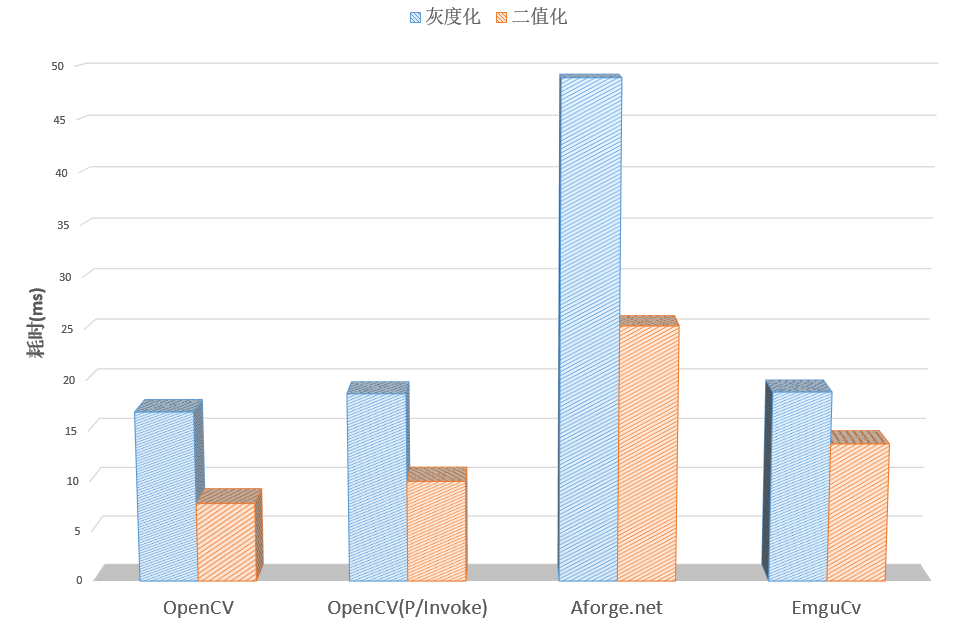
\includegraphics[width=0.9\textwidth]{Image-Processing-Comparison}
	\caption{几种图像处理库的性能比较}
	\label{pic:image-processing-comparison}
\end{figure}

OpenCV(Open Source Computer Vision)是一个旨在完成实时机器视觉(Real-time Computer Vision)的函数库,最早是由英特尔研究中心开发,后被Will Garage接手,现在是由Itseez团队负责维护,是一个跨平台的免费开源图像处理库\citep{wiki:OpenCV}。OpenCV最早于2000年发行,目前仍在更新和维护,最新的稳定版是于2015年12月发布的OpenCV 3.1更新。它的代码由C/C++写就,同时提供了Python、Java以及Matlab等语言的接口\citep{wiki:OpenCV}。自其发布后的15年来,OpenCV一直以它良好的性能和高度的稳定性著称,是使用最为广泛的图像处理库。这也意味着它有着大量的用户测试经验和成熟的社区支持,这无疑为我们解决项目中的棘手问题提供了基础保障,具体来说,本系统的数据加载模块、版面分析模块、预处理模块都需要用到OpenCV提供的函数方法支持,我们也将在后面的模块详细介绍中,体会到OpenCV的强大功能。

\subsubsection{环境部署}
OpenCV是有很好的多平台支持(Windows,Linux,Mac等),环境的部署也比较简单,这里我们仅以Windows平台下Visual Studio 2013的opencv配置使用为例,做一个部署步骤的简要展示:
\begin{itemize}
  \item 从\href{http://opencv.org/}{OpenCV官方主页}下载最新的OpenCV 3.1安装包,解压安装包完成安装。并将OpenCV加入系统环境变量。
  \item 新建一个Visual Studio C++工程,在工程配置属性中的“包含目录”中添加OpenCV的include文件夹,在“库目录”中加入OpenCV的lib文件夹,在“链接器”的附加依赖中添加opencvworld310d.lib和opencvworld310.lib(分别对应debug和release编译选项)。
  \item 在工程中添加如下测试代码OpenCV-test.cpp(代码见下方,功能是展示示例图片),编译运行,如果编译通过,并且程序正确开辟“example”窗口并显示示例图片,说明OpenCV的环境就配置成功了。
\end{itemize}

\begin{Codex}[label=OpenCV-test.cpp, numbers=left]
#include <iostream>
#include "opencv2/highgui/highgui.hpp"
using namespace cv;
int main(void)
{
  Mat img = imread("example.jpg", 0);
  imshow("example", img);
  waitKey();
  return 0;
}
\end{Codex}

上面只是简述了OpenCV的部署步骤,具体到不同的平台和软件版本,部署时会有一些小的差异,读者可结合自己的情况,从网络上找到对应的详细部署指南,这里就不再赘述了。

\subsection{字符识别}
\subsubsection{方案选取}
字符识别(Character Recognition),又称光学字符识别(Optical Character Recognition,OCR),是指将印刷或手写的文字转换成机器编码(machine-encoded)文本的过程,它被广泛应用于纸质印刷的数据录入中,例如护照文件、发票、信件、银行存单等,当这些纸质文件被转换成了机器编码的文本以后,无论是在编辑修改、搜索、存储,还是在后续的数据挖掘,文字转语音等过程中,都变得相对便捷和高效。OCR是模式识别(Pattern Recognition)、(Artificial Intelligence)和计算机视觉(Computer Vision)领域中的典型应用\citep{wiki:OCR}。

具体到本系统,我们是要讲光学字符识别技术应用到纸质或截图保存的病历数据中,这项技术会在OCR模块中用到,在技术实现上与其他基于光学字符识别的应用并没有本质的不同,因此我们可以采用已有的OCR解决方案。目前比较主流的OCR解决方案有ABBYY FineReader、Microsoft Office内置的OCR模块、Tesseract、FreeOCR等,维基百科中有对各种OCR软件的详细对比\citep{wiki:OCRcomparison},同时,也有组织对于最好的OCR软件做过一个排名(见\autoref{pic:ocr-software-comparison}),从这个排名中我们可以看到,好的商用OCR软件一般都售价不菲(图片中的价格仅针对个人用户),同时由于病历数据的版面结构复杂,并没有一个比较通用的版面分析方案,所以这些商用OCR软件无法直接应用到系统中,因此,我们需要一个有提供编程接口(Application Programming Interface,API)的OCR解决方案,方便定制特定场景下的OCR。能提供编程接口的OCR引擎中,Tesseract是其中的首选。

\begin{figure}
	\centering
	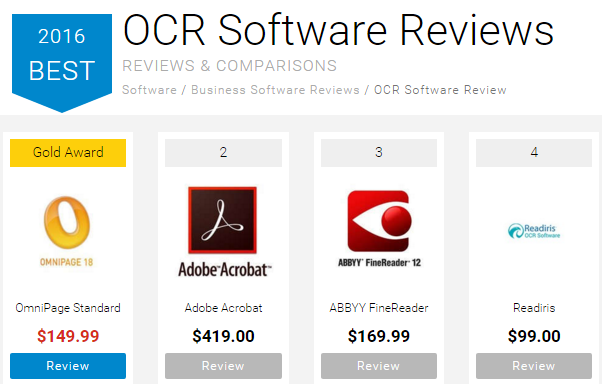
\includegraphics[width=0.9\textwidth]{ocr-software-comparison}
	\caption{某组织对现有OCR软件的排名}
	\label{pic:ocr-software-comparison}
\end{figure}

Tesseract OCR引擎是一款能运行在多系统全平台(Windows,Linux,Mac,IOS,Android)的免费开源OCR引擎,最早由惠普公司Hewlett Packard实验室的工程师在1985年到1994年间开发和维护,并于2005年开放源代码,2006年之后由谷歌公司接手开发和维护\citep{wiki:Tesseract}。

在1995年,Tesseract在识别准确率上是排名前三的OCR引擎,最早的版本只支持英文,之后逐步添加多语言的支持,其中就包括中文。准确性较高、支持多语言加之免费开源,使得Tesseract在这些年,广受赞誉,是公认最好的开源OCR引擎,读者可访问\href{https://github.com/tesseract-ocr/tesseract}{Tesseract的GitHub主页}来获取最新的源代码。同时,Tesseract的源码是由C/C++编写,与同样是C/C++编写的OpenCV图像处理库能够很好的兼容,事实上,Tesseract也开发了专门针对OpenCV的API接口,提供了丰富的支持。综上,系统决定采用Tesseract作为字符识别的解决方案。

\subsubsection{环境部署}
Tesseract支持多平台(Windows,Linux,Mac)使用和开发,如果只是简单使用tesseract,可以下载安装包安装Tesseract的可执行程序,如果需要基于Tesseract进行二次开发,则需要编译它的源代码,显然,我们的需求属于后者。接下来本文以Windows平台下Visual Studio 2013的Tesseract编译为例,做一个简要的环境部署展示:
\begin{itemize}
	\item 安装版本控制软件Git\footnote{更多相关信息可访问Git官方网站:https://git-scm.com/}。
	\item 在电脑中建立tesseract-build文件夹,在该文件夹下打开CMD控制台程序,并分别运行:
	\begin{Code}[numbers=left]
git clone git://github.com/charlesw/tesseract-vs2012.git
git clone git://github.com/tesseract-ocr/tesseract.git
	\end{Code}
	\item 打开VS 2013 Developer Command Prompt,然后输入命令:
	\begin{Code}[numbers=left]
msbuild "${tesseract-build}\tesseract-vs2012\build.proj"
	\end{Code}
	其中\$\{tesseract-build\}表示tesseract-build这个文件夹在电脑中的绝对路径。
	\item 将vs2013+64bit\_support.batch文件拷贝到tesseract-build文件夹下,然后进入到tesseract文件夹,执行以下命令:
	\begin{Code}[numbers=left]
git checkout -b 3.04-vs2013 3.04.00
git am --signoff ../vs2013+64bit_support.patch
	\end{Code}
	\item 将tesseract-build$\backslash$tesseract-vs2012$\backslash$release目录下的所有文件拷贝到tesseract-build目录下。
	\item 用VS2013打开tesseract-build$\backslash$tesseract$\backslash$vs2013下的tesseract.sln工程,开始编译,如果编译正常通过,就说明环境已经配置完成。
\end{itemize}

上面的只是一个配置过程的简述,不同平台、不同版本之间的配置方式有着比较明显的差异,需结合自身的情况,选取对应的配置部署流程,这里不再详述。

\section{数据加载模块}  %500字
可添加简单的容错处理

\section{版面分析模块}  % 3000字
文档版面分析(Document Layout Analysis),是指在含有文本的图像中识别出感兴趣区域(Regions of Interest,ROI)的过程。一个文字识别系统需要将文字从非文字的区域中划分出来,同时保持文本的相对顺序\citep{baird1992anatomy}。在一个文件中检测和标记出文本区域和其他非文本区域的过程叫做几何学版面分析(Geometric Layout Analysis)\citep{cattoni1998geometric}。但是不同的文本区域在文档中代表的含义并不相同,例如有些文本是文档的标题,有些是文档的注释,有些是文档的主体等等,具体到病历档案归类系统中,就是文本块所属的字段是各不相同的,这种识别文字在文档中的含义的过程叫做逻辑学版面分析(Logical Layout Analysis)\citep{haralick1994document}。

(几何学)版面分析算法总体上可以分为三类\citep{mao2003document}:
\begin{itemize}
	\item 自顶向下方法,算法从整张图片开始,迭代地将图片不断分割成更小的区域,直到程序达到某种终止条件时停止。它的优点是操作简单、速度较快,但是难以适应比较复杂的版面\citep{nagy1992prototype}\citep{baird1990image}。
	\item 自底向上方法,与自顶向下的方法相反,算法从每一个图片像素开始,根据一定的聚即规则,逐渐聚集相邻的区域形成单词,语句和段落。它的优点是能够适应比较复杂的版面,缺点是速度比较慢,难以确定一个比较好的聚集规则\citep{o1993document}\citep{kise1998segmentation}。
	\item 混合型方法,它可以被看做是自顶向下和自底向上这两种方法的混合\citep{pavlidis1992page}。
\end{itemize}

在真实的应用场景中,由于实际文档的多样性,复杂性,因此,目前还没有一个固定的,最优的切割模型,需要我们根据实际问题和需求,有针对性的设计版面分析方法。在\autoref{ssec:framework-segmentation-analysis}中我们已经提到,系统的版面分析模块非常重要,需要完成以下三大功能:
\begin{itemize}
	\item 对病历图片进行二次分类;
	\item 剔除图片中的干扰信息,获得病历数据主体;
	\item 剔除主体内容中的空白,提取出各个字段。
\end{itemize}
这三个功能我们可以简单归纳为图片分类、主体保留、字段提取。这三者的顺序是从逻辑上出发来区分的,在实际代码实现中,我们是先实现了主体保留,此时再对图片分类,最后做字段提取的工作。接下来,我们分别讨论这三个功能如何实现。

\subsection{主体保留}
图片中除了我们需要的病历主体信息以外,一般还会有冗余的干扰信息,以\autoref{pic:input-image-1}为例,图片的中间部分是病人病历数据的主体,而图片上部则是一些电子病历系统的系统信息,左侧则是一个侧边栏导航,这些都是与病历无关的,我们需要将其剔除,保留主体,这里需要用到图片的裁剪。

\subsubsection*{OpenCV中矩形框裁剪}
在OpenCV中,可以很方便的根据矩形框来裁剪,假如原始图片已转换为Mat格式\footnote{Mat是OpenCV 2.x中图片加载以后的格式},名字为origin,我们需要产生的裁剪图片为cut,那么裁剪的代码为:
\begin{Code}
cut = origin( Rect(x0, y0, width, height) );
\end{Code}
其中$(x_0,y_0)$表示裁剪区域的左上角在原图中的位置,width和height则分别表示裁剪区域的宽度和高度。

现在我们知道用OpenCV裁剪矩形图片了,但是对于\autoref{pic:input-image-1}这样的数据,我们怎么确定$(x_0,y_0)$和width、height呢?

\subsubsection*{模板匹配}
需要注意的是,在确定的病历系统中,其系统信息和侧边栏导航的内容和位置是相对固定的,我们可以根据这一点,利用模板匹配的方式,确定系统信息栏和侧边导航栏的位置,并进行裁剪。

模板匹配(Template Matching)\citep{template-matching},是一项在原始图片中寻找匹配模板图片的小区域的技术。在OpenCV中,提供了模板匹配的函数
\begin{Code}
void matchTemplate(InputArray image, InputArray templ, OutputArray result, int method)
\end{Code}
其中image表示原始图像,templ表示模板图像,result为结果矩阵,method为匹配算子类型。具体匹配过程为模板图像在原始图像中滑动,根据不同的匹配算子,计算重叠区域的匹配度,当滑动过整个原始图像区域后,返回匹配度最高的子图像信息。

OpenCV提供了6种默认的匹配算子,最常见的是平方差匹配算子(\autoref{eq:square})和相关匹配算子(\autoref{eq:correlation}):
\begin{equation} \label{eq:square}
R(x,y)=\sum_{x^{'},y^{'}}(T(x^{'},y^{'})-I(x+x^{'},y+y^{'}))^2
\end{equation}

\begin{equation} \label{eq:correlation}
R(x,y)=\sum_{x^{'},y^{'}}(T(x^{'},y^{'})\cdot I(x+x^{'},y+y^{'}))
\end{equation}
其中,$T(x^{'},y^{'})$表示模板图像中的点,$I(x+x^{'},y+y^{'})$表示原始图像滑动窗口中对应的点。平方差匹配算子衡量的是两者的差别,所以这个值越低,说明匹配度越高,而相关匹配算子衡量的是两者的相关性,所以这个值越高,说明匹配度越高。

\begin{figure}
	\centering
	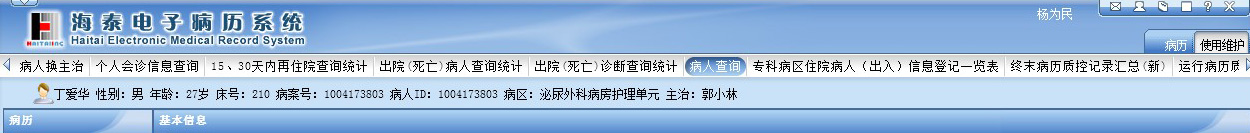
\includegraphics[width=0.9\textwidth]{title-template}
	\caption{系统信息栏模板}
	\label{pic:title-template}
\end{figure}

对于病历图片中的系统信息栏,我们可以通过截取原图中系统信息栏的部分保存下来,作为模板,如\autoref{pic:title-template}所示。然后运用模板匹配算法,剪裁掉原图中上方系统信息栏部分,代码如下:(其中算子采用平方差算子,输入参数src代表原图,\_template代表模板,template\_type为模板类型,返回值roi为截掉模板之后的图像。)
\begin{Codex}[label=Cut,numbers=left]
Mat MatchingMethod(Mat src, Mat _template, int template_type)
{
	// template_type option:  0 -> title, 1 -> sidebar
	Mat result;
	int match_method = CV_TM_SQDIFF_NORMED;
	Mat img_display;
	src.copyTo(img_display);
	int result_cols = src.cols - _template.cols + 1;
	int result_rows = src.rows - _template.rows + 1;
	result.create(result_rows, result_cols, CV_32FC1);
	matchTemplate(src, _template, result, match_method);
	normalize(result, result, 0, 1, NORM_MINMAX, -1, Mat());
	double minVal; double maxVal; Point minLoc; Point maxLoc;
	Point matchLoc;
	minMaxLoc(result, &minVal, &maxVal, &minLoc, &maxLoc, Mat());
	matchLoc = minLoc;
	Mat roi;
	if (template_type)
	roi = src(Rect(matchLoc.x + _template.cols, matchLoc.y, src.cols - matchLoc.x - _template.cols, _template.rows));
	else
	roi = src(Rect(0, matchLoc.y + _template.rows, matchLoc.x + _template.cols, src.rows - matchLoc.y - _template.rows));
	return roi;
}
\end{Codex}

去掉系统信息栏之后的图像如\autoref{pic:template-cut-title}所示,接着我们采用同样的方法,也可去掉侧边的导航栏,最终得到\autoref{pic:template-cut-title}所示,可以看到,病历的主体已经被完整的剥离出来,至此,主体保留的工作就完成了。

\begin{figure}[htbp]
  \centering
  \subfloat[]{
  \label{pic:template-cut-origin}
  \begin{minipage}[t]{0.3\textwidth}
    \centering
    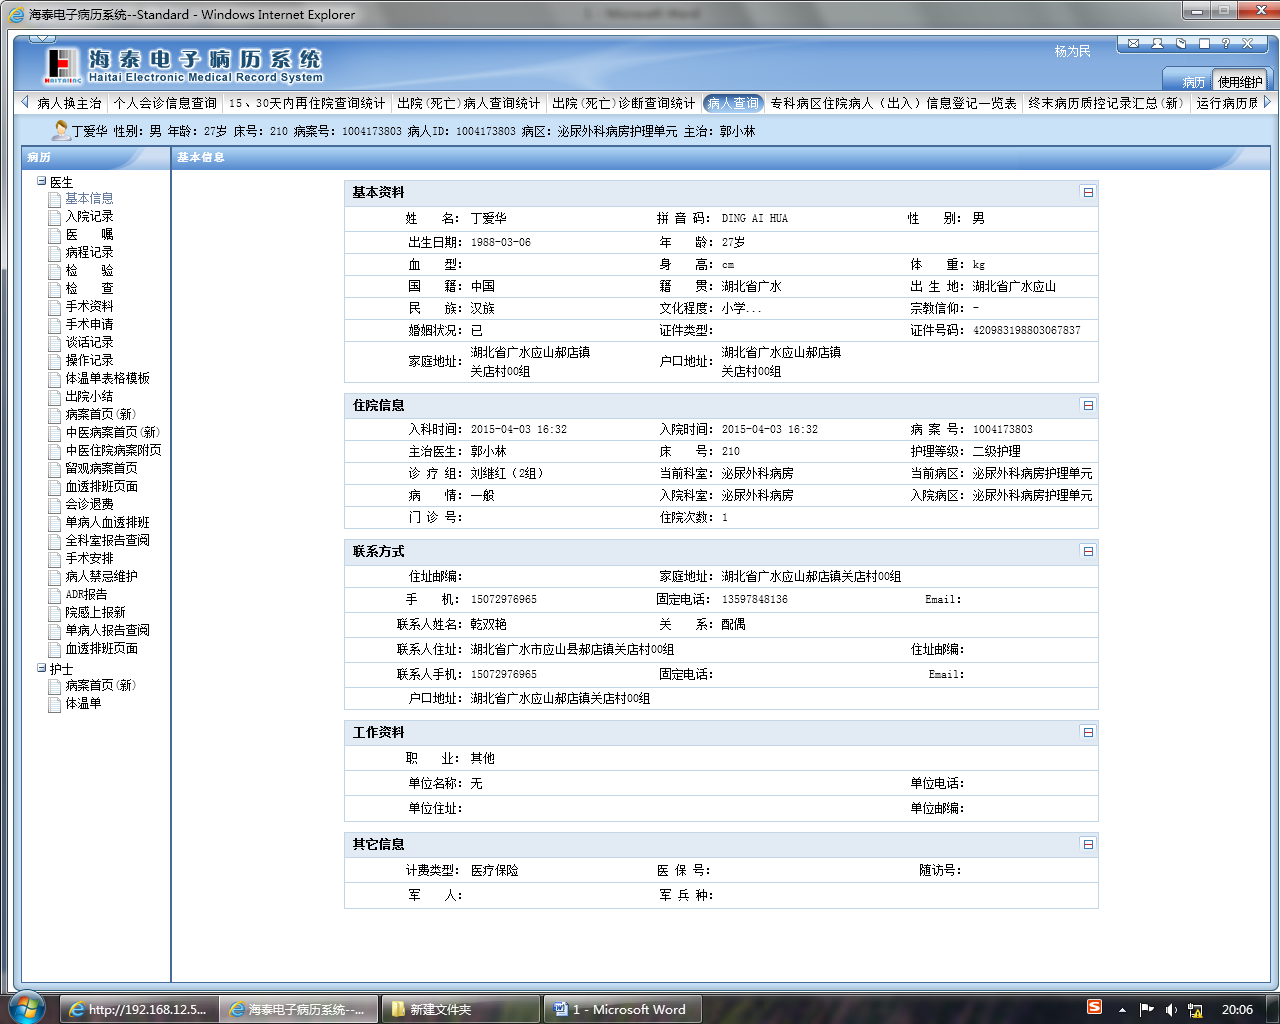
\includegraphics[width=\textwidth]{input-image-1}
  \end{minipage}
  }
  \subfloat[]{
  \label{pic:template-cut-title}
  \begin{minipage}[t]{0.3\textwidth}
    \centering
    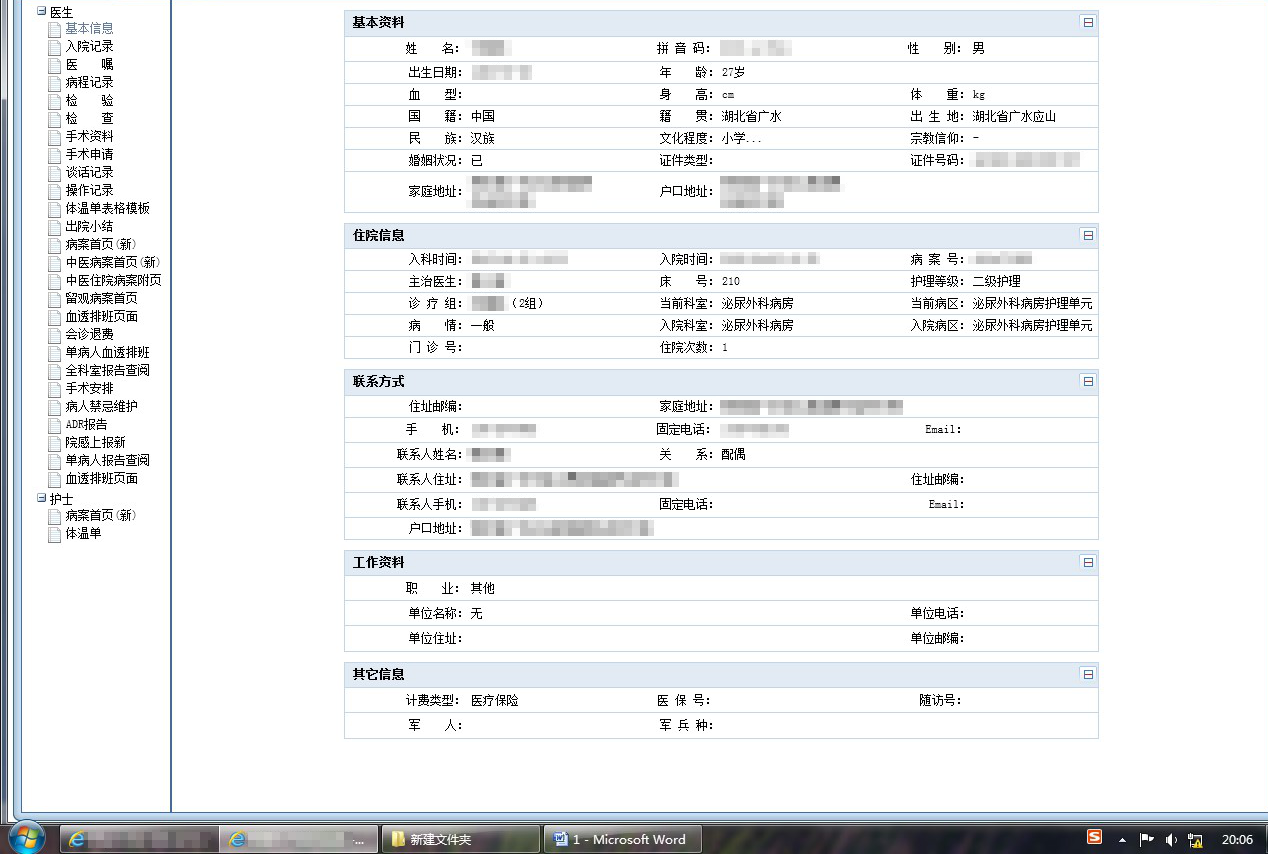
\includegraphics[width=\textwidth]{cut_title}
  \end{minipage}
  }
  \subfloat[]{
  \label{pic:template-cut-sidebar}
  \begin{minipage}[t]{0.3\textwidth}
    \centering
    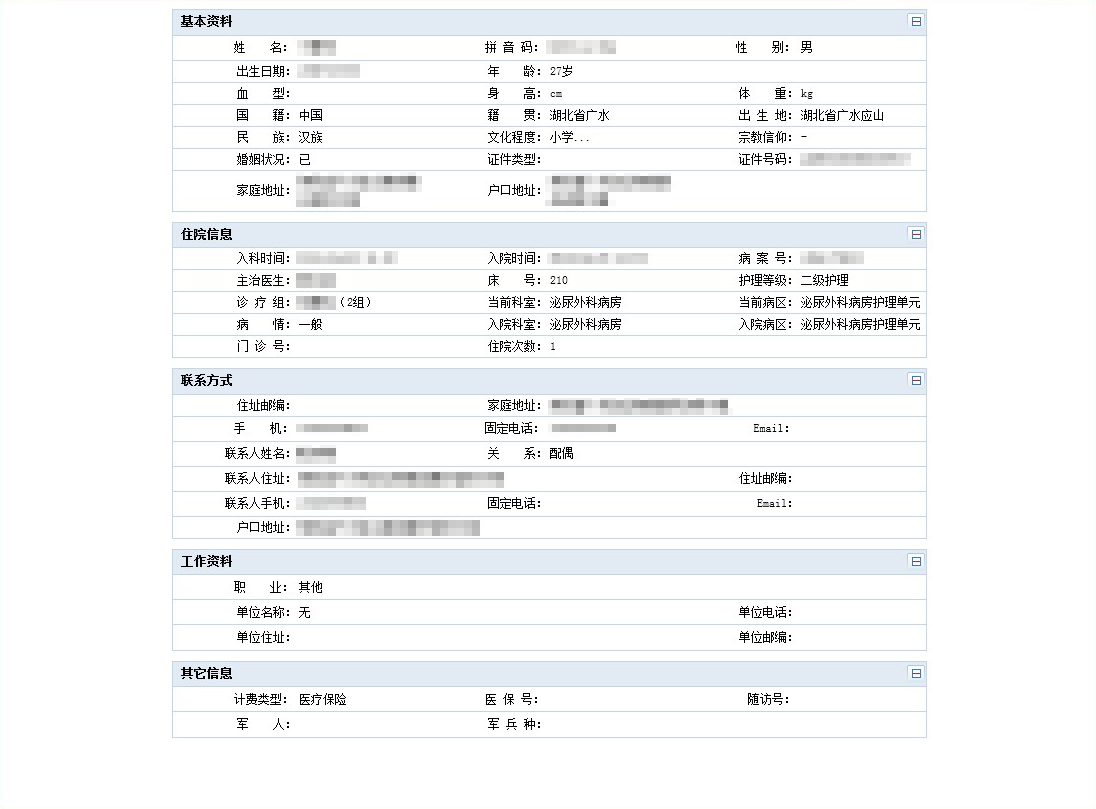
\includegraphics[width=\textwidth]{cut_sidebar}
  \end{minipage}
  }
  \caption{病历主体内容截取}
  \label{pic:different-layout}
\end{figure}

\subsection{图片分类}
在\autoref{ssec:framework-segmentation-analysis}中,我们已经提到每个病人对应着大约7到10张图片,这些图片的内容互不重复,加起来构成了完整的病人诊疗信息,图片之间的版式是各不相同的,如\autoref{pic:different-layout}所示,三张图片都属于同一个病人的病历数据,但是主体内容的版式各不相同,\autoref{fig:sub-input-image-1}中主要记录的是病人的基本信息,如姓名、性别等,\autoref{fig:sub-input-image-3}中记录的则是病人详细的病情数据,而\autoref{fig:sub-input-image-2}则介于两者之间。假设病人的病历图片只有这三种样式,那么当有一张图片输入时,应该如何判断这张图片属于哪个样式呢?这就涉及到图片相似度(image similarity measure)度量的问题了。

\begin{figure}[htbp]
  \centering
  \subfloat[]{
  \label{fig:sub-input-image-1}
  \begin{minipage}[t]{0.3\textwidth}
    \centering
    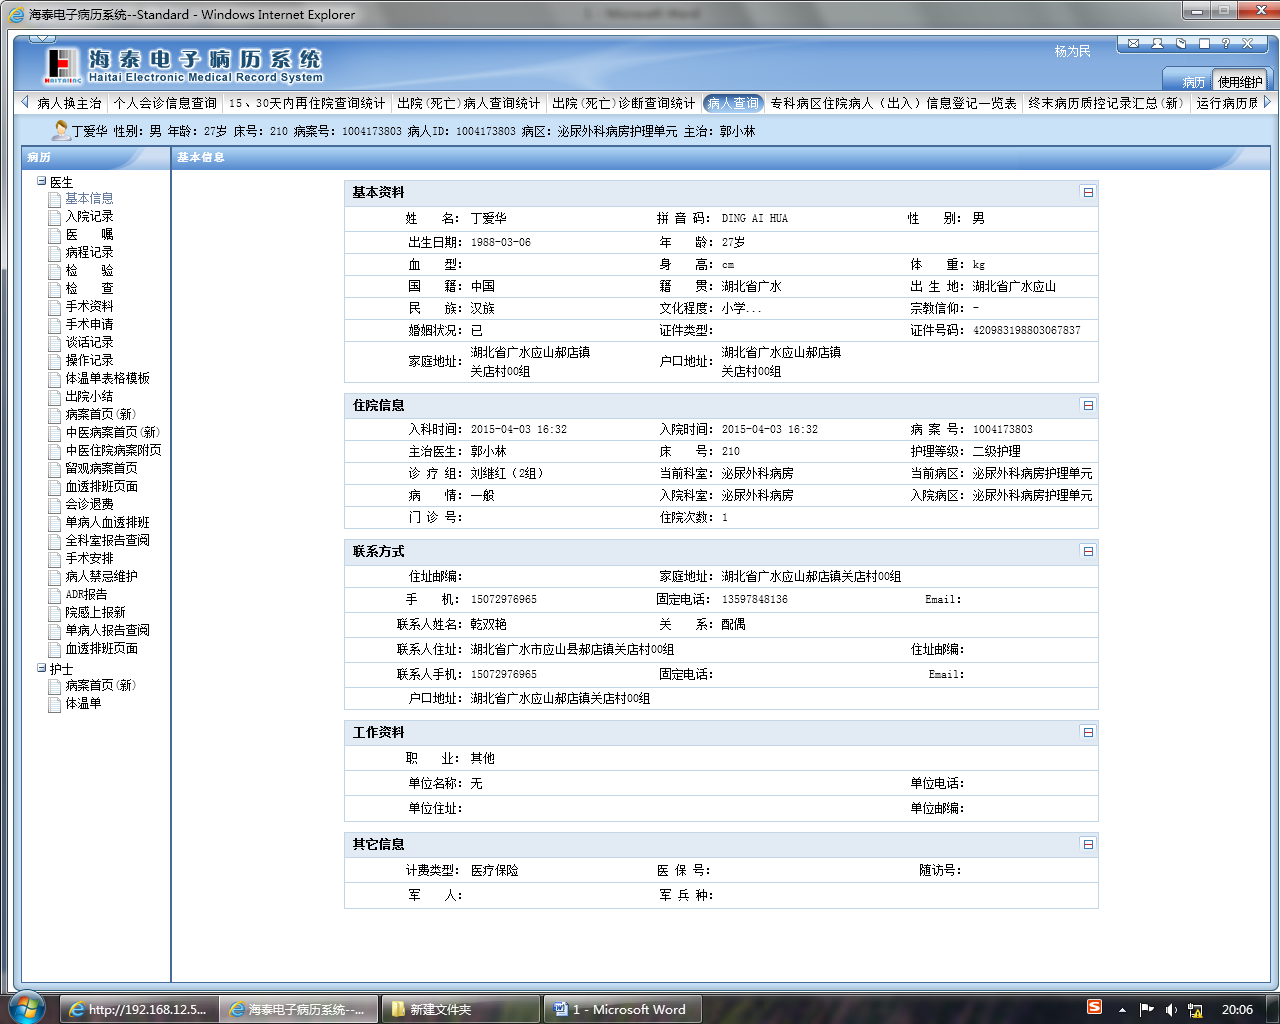
\includegraphics[width=\textwidth]{input-image-1}
  \end{minipage}
  }
  \subfloat[]{
  \label{fig:sub-input-image-2}
  \begin{minipage}[t]{0.3\textwidth}
    \centering
    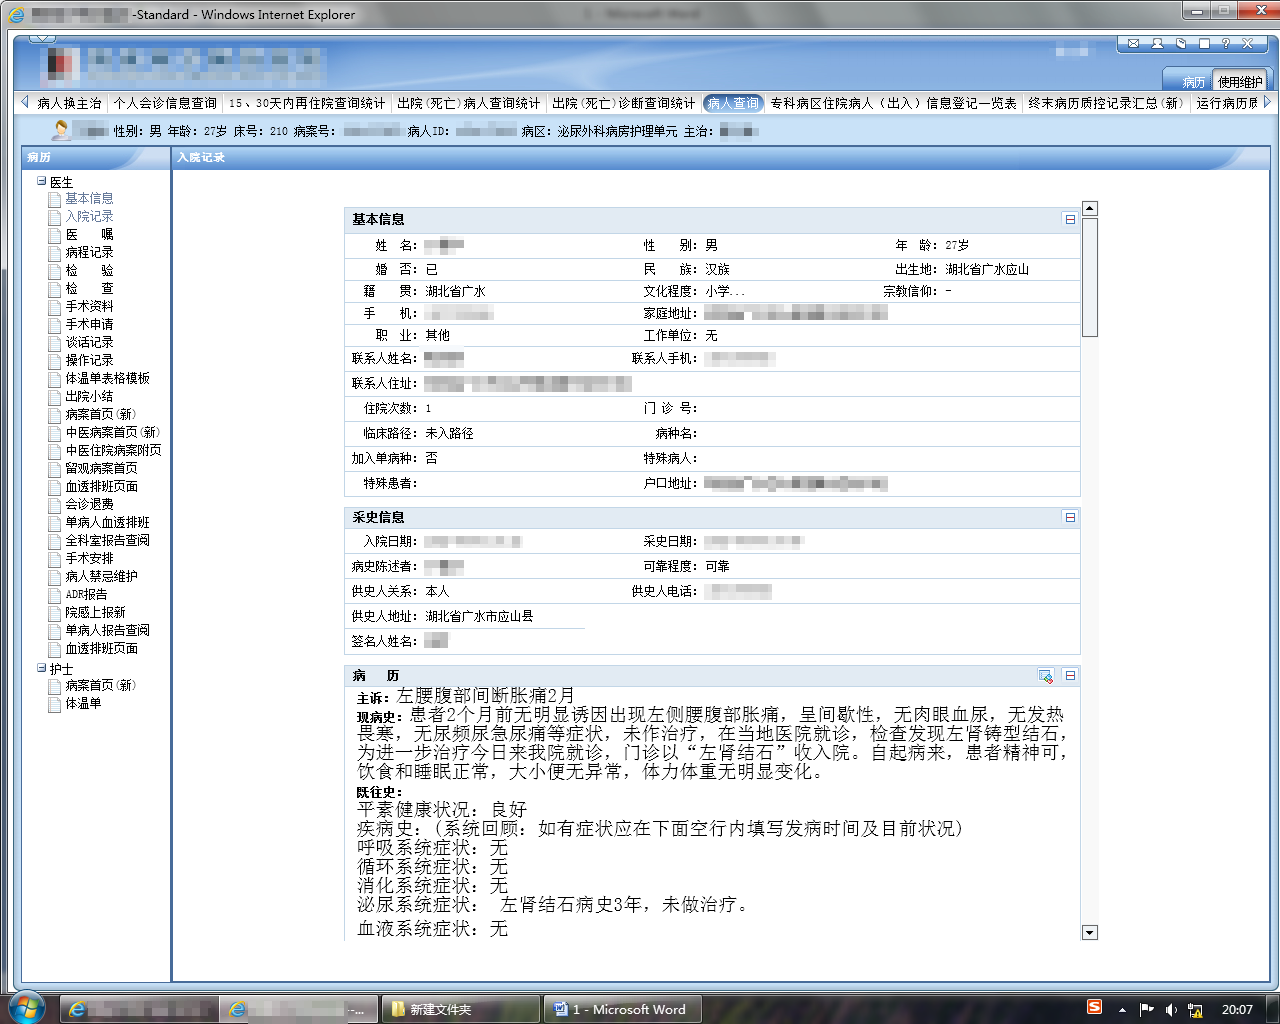
\includegraphics[width=\textwidth]{input-image-2}
  \end{minipage}
  }
  \subfloat[]{
  \label{fig:sub-input-image-3}
  \begin{minipage}[t]{0.3\textwidth}
    \centering
    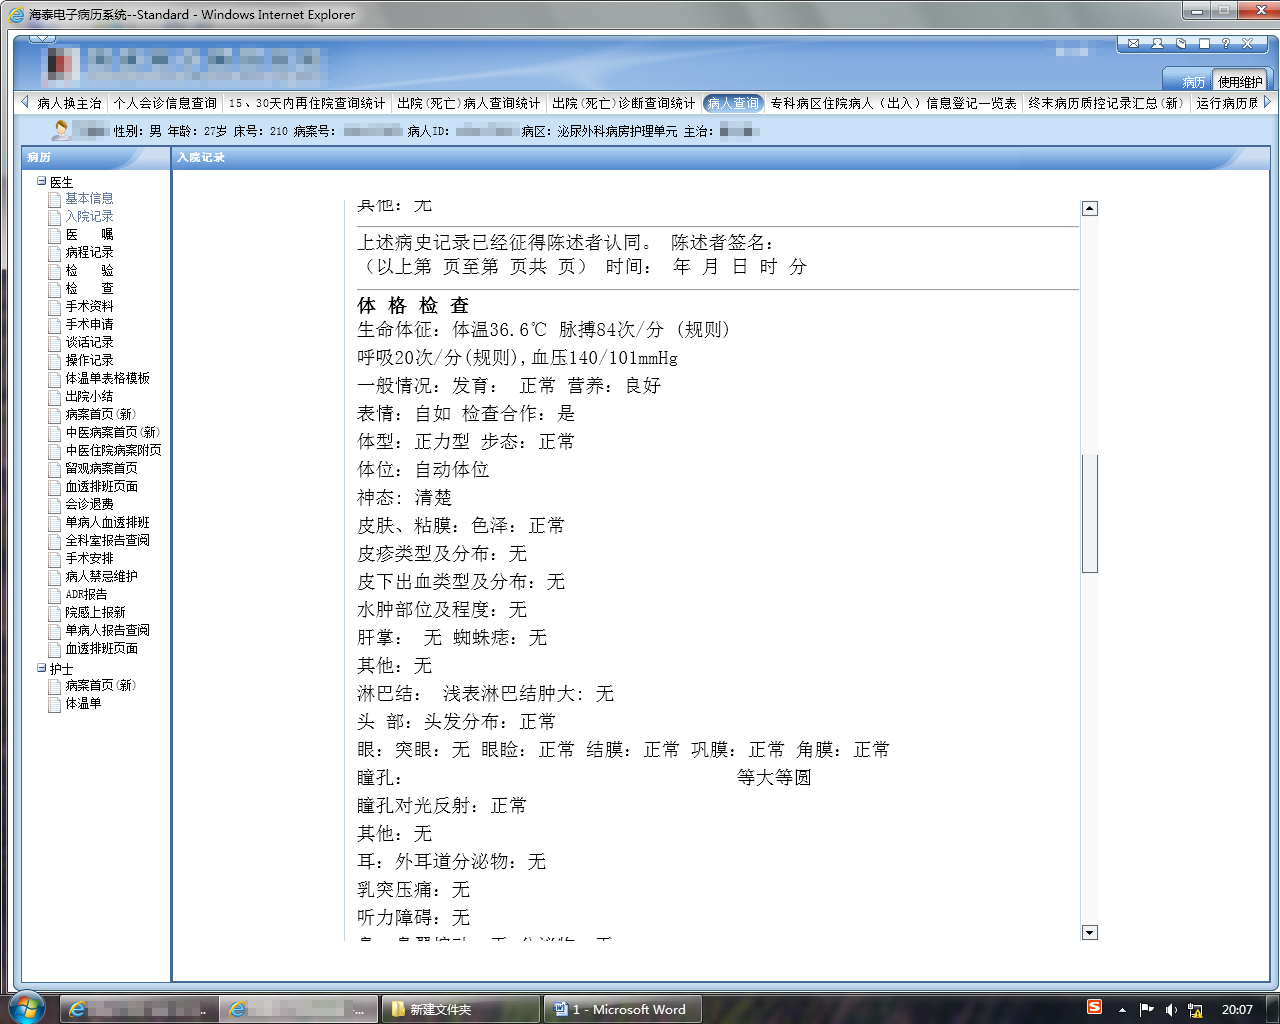
\includegraphics[width=\textwidth]{input-image-3}
  \end{minipage}
  }
  \caption{病历图片的几种版式}
  \label{pic:different-layout}
\end{figure}

相似性度量(Similarity Measure)\citep{lin1998information},或者距离度量(Distance Meature),是一个用来定义两个物体相似性或者距离的实值函数\citep{singhal2001modern},常见的相似性度量函数有欧几里得距离(Euclidean distance)\citep{wiki:Euclidean-distance}、余弦距离(Cosine Distance)\citep{wiki:Cosine-distance}、机器学习中的核函数(Kernel Functions)\citep{hofmann2008kernel}等等,这些相似性度量在数据挖掘领域有着广泛的应用\citep{tan2006introduction}。图片相似度度量,是相似性度量的一个特例,当然,版式作为图片信息的一个抽象,它的相似度度量是图片相似度度量的一个子集。一般来说,图像相似性度量分为两个部分\citep{goldberger2003efficient}:
\begin{itemize}
  \item 图像表示(Image Representation),既然相似性度量是一个实值函数,那么图片数据需要转换成某种数值的表示形式才能进行度量,比较常见的表示方法是将图片中的每个像素分成红绿蓝三个维度的0-255的整数值进行存储,而灰度、二值等都是不同的图片表示方法。
  \item 相似度定义与计算,定义一个合适的相似度度量指标,计算图片间的相似度。这个是与问题相关的,不同问题适用的相似度度量也不一样。
\end{itemize}
具体到病历图片版面相似性度量,由于我们的病历图片的版式只有固定的几种,假设为三种,这样对于每张图片,我们可以与这三种版式分别进行相似性比较,相似度最高的就是该图片的版式。但是对于同一种版式,各个字段的内容是不相同的,比如姓名字段,每个病人的名字就各不相同,因此,我们需要预先对图片做一些处理,抛弃一些细节信息,消除因为各个字段内容不同造成的整体相似度的差异。这里就需要用到图像处理中图片的灰度化、二值化、腐蚀等操作了,我们先来逐一介绍下这几种图像转换方法。

\subsubsection*{灰度化}
\label{sub:灰度化}
一张彩色图像在计算机中是由若干个像素点的形式存在,像素点的多少取决于图像的分辨率PPI(Pixel Per Inch),而每个像素点最常见的表示形式是RGB(Red,Green,Blue,即红。绿。蓝)三原色,三原色的不同组合比例能表示丰富的色彩。而灰度图(Greyscale Image)则是另外一种表示形式,它只保存了每个像素的亮度(Intensity)信息,将RGB图像转换为灰度图需满足\autoref{eq:RGBtoGray}:
\begin{equation} \label{eq:RGBtoGray}
		\begin{split}
& P(x,y) = \alpha R(x,y) + \beta G(x,y) + \gamma B(x,y),  \\
& where \quad \alpha,\beta,\gamma > 0,\alpha + \beta + \gamma = 1
		\end{split}
\end{equation}
其中,$P(x,y)$表示像素点的灰度值,$R(x,y),G(x,y),B(x,y)$表示像素点的三原色值,系数$\alpha,\beta,\gamma$的一个常见取值为$\alpha=0.299,\beta=0.587,\gamma=0.114$。从\autoref{eq:RGBtoGray}中我们可以知道,灰度转换实际上是从RGB三维到灰度一维的投影,这种转换会损失信息,并且是不可逆的。\autoref{pic:greyscale}展示了RGB图像灰度化以后的结果。

\begin{figure}[htbp]
  \centering
  \subfloat[]{
  \label{pic:lena}
  \begin{minipage}[t]{0.45\textwidth}
    \centering
    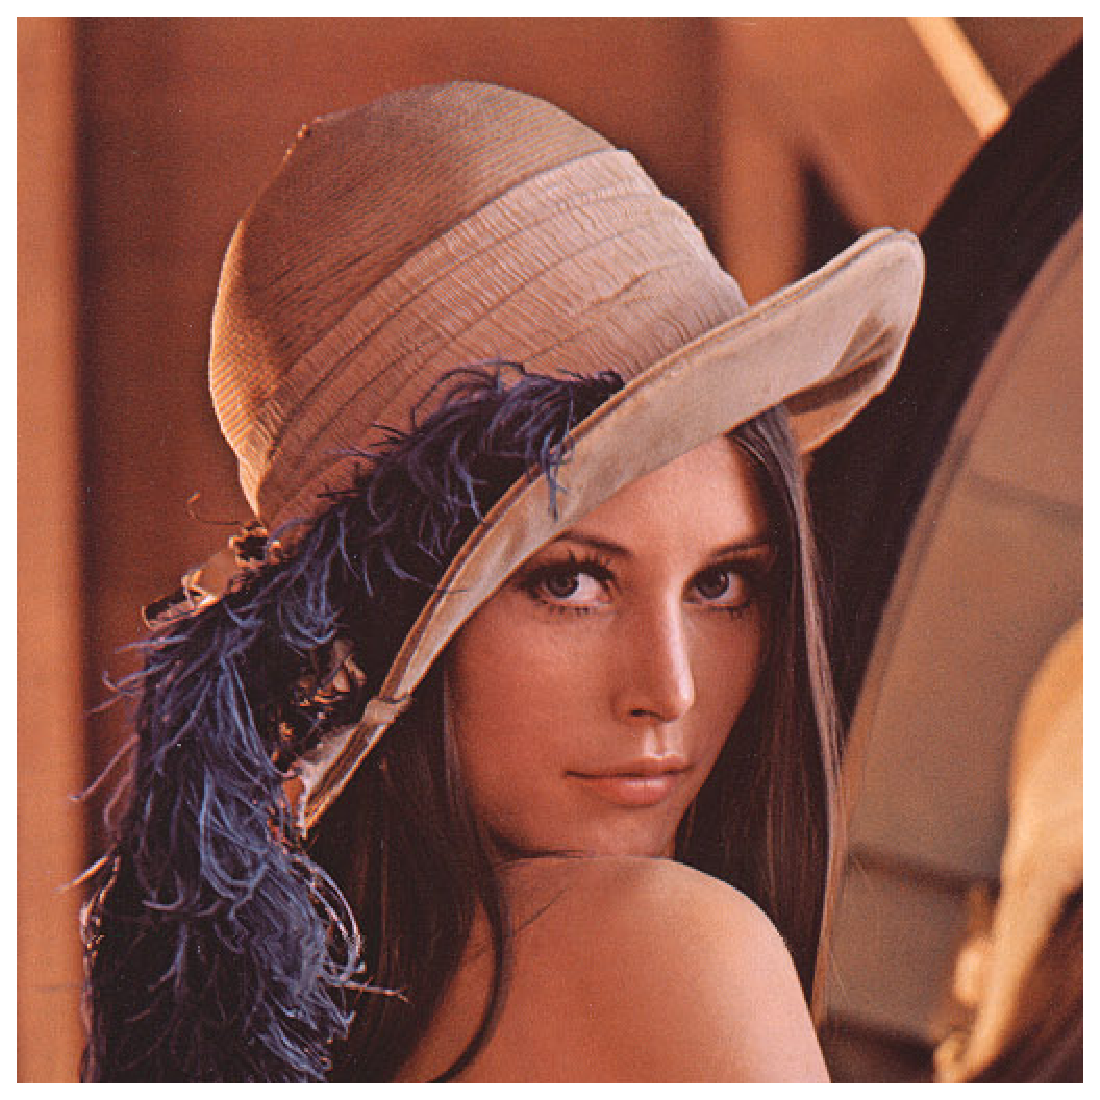
\includegraphics[width=\textwidth]{lena}
  \end{minipage}
  }
  \subfloat[]{
  \label{pic:lena-grey}
  \begin{minipage}[t]{0.45\textwidth}
    \centering
    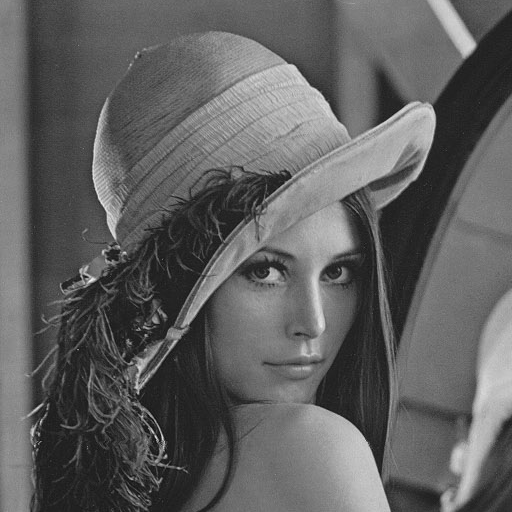
\includegraphics[width=\textwidth]{lena_grey}
  \end{minipage}
  }
  \caption{图片的灰度化}
  \label{pic:greyscale}
\end{figure}

\subsubsection*{二值化}
\label{sub:二值化}
二值化图像(Binary Image)中,每个像素只有两种可能的值,分别是黑和白,将灰度图二值化的过程满足\label{pic:binarization}:
\begin{equation} \label{pic:binarization}
	B(x)=
	\begin{cases}
		0,&x\geq threshold\cr 1,&x<threshold
	\end{cases}
\end{equation}
其中$x$表示像素点的灰度值(常见取值为$0-255$),$threshold$为二值化的阈值,当$x$大于阈值时,该像素点为白色,反之为黑色。OpenCV提供了两种二值化方法,分别是固定阈值方法和自适应阈值方法。

固定阈值方法,即需要事先指定一个全局阈值,根据这个阈值对灰度图进行二值化,函数原型为
\begin{Code}
double threshold(InputArray src, OutputArray dst, double thresh, double maxval, int type)
\end{Code}
固定阈值方法虽然实现简单,但是阈值需要人工选取,很难保证效果,当阈值选的太大时,会产生很多噪声,淹没主体(见\autoref{lena_binary_130}),阈值选的太小时,又会丢失大量的细节(见\autoref{lena_binary_70}),因此这种方法在具体实施时并不推荐。

自适应阈值方法,函数原型为
\begin{Code}
void adaptiveThreshold(InputArray src, OutputArray dst, double maxValue, int adaptiveMethod, int thresholdType, int blockSize, double C)
\end{Code}
它根据像素的邻域块的像素值分布来确定该像素位置上的二值化阈值。这样做的好处在于每个像素位置处的二值化阈值不是固定不变的,而是由其周围邻域像素的分布来决定的。亮度较高的图像区域的二值化阈值通常会较高,而亮度较低的图像区域的二值化阈值则会相适应地变小。不同亮度、对比度、纹理的局部图像区域将会拥有相对应的局部二值化阈值。常用的局部自适应阈值有:1)局部邻域块的均值;2)局部邻域块的高斯加权和。%这一段摘自http://blog.csdn.net/icvpr/article/details/8515596
自适应阈值二值化效果见\autoref{lena_binary_adaptive},图片即保证了主体的明确,没有很多噪声,又保留了大部分的细节。

\begin{figure}[htbp]
  \centering
  \subfloat[]{
  \label{pic:lena_binary_origin}
  \begin{minipage}[t]{0.3\textwidth}
    \centering
    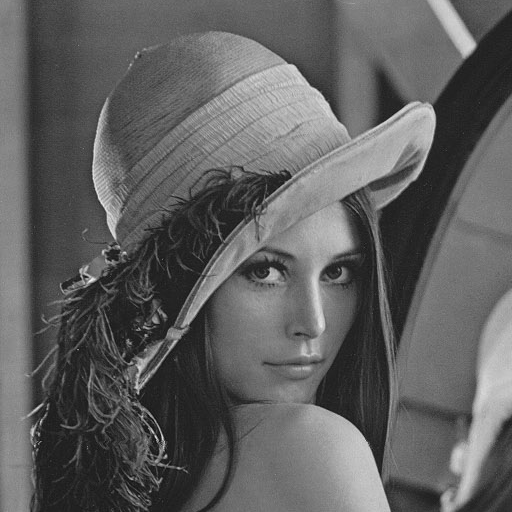
\includegraphics[width=\textwidth]{lena_grey}
  \end{minipage}
  }
  \subfloat[]{
  \label{pic:lena_binary_130}
  \begin{minipage}[t]{0.3\textwidth}
    \centering
    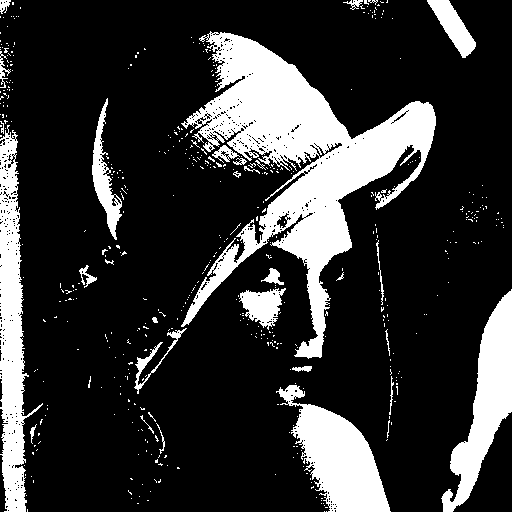
\includegraphics[width=\textwidth]{lena_binary_130}
  \end{minipage}
  }
  \subfloat[]{
  \label{pic:lena_binary_70}
  \begin{minipage}[t]{0.3\textwidth}
    \centering
    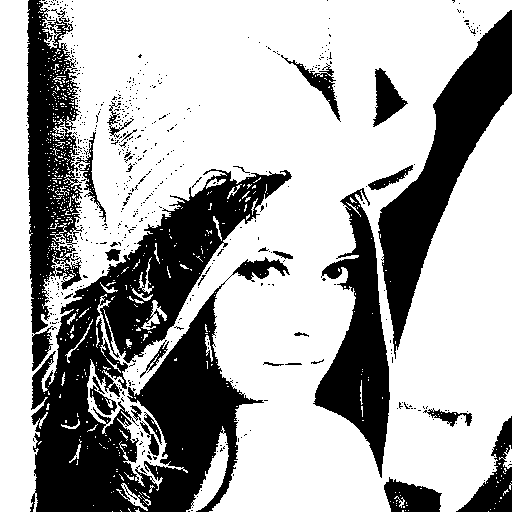
\includegraphics[width=\textwidth]{lena_binary_70}
  \end{minipage}
  }
  \subfloat[]{
  \label{pic:lena_binary_adaptive}
  \begin{minipage}[t]{0.3\textwidth}
    \centering
    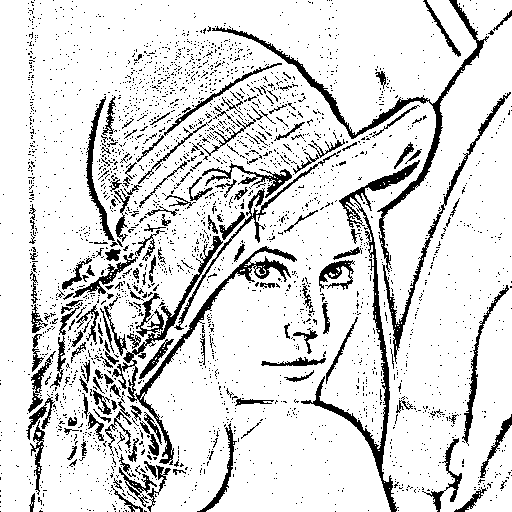
\includegraphics[width=\textwidth]{lena_binary_adaptive}
  \end{minipage}
  }
  \caption{不同二值化方法的差别}
  \label{pic:different-binary-approach}
\end{figure}

\subsubsection*{图像的膨胀和腐蚀}
图像的膨胀和腐蚀是两种常见的图像形态学操作(Morphological Operations),形态学操作简而言之,就是根据一个结构化元素(Structuring Element)对输入图片进行一系列基于外形的图像处理操作,得到输出图片。图像的膨胀和腐蚀在很多方面都有应用,例如去噪、个体元素提取或连接等。

膨胀(Dilation),可以被看做一个是基于某个核(Kernel)$B$的卷积(convoluting)操作,这个核$B$可以是任意的形状和大小,一般来说是方形或者是原型,
核$B$一般有一个预先定义好的锚点(anchor point),一般来说是核的中心。当核$B$依次扫过图片的时候,在$B$与图片的重叠区域,算法会计算区域内的最大值,并将当前锚点的值替换为这个最大值,显然,这样的最大化操作会使图片中比较亮的区域扩张,如\autoref{pic:dangan}中,\autoref{pic:dangan_origin}是包含有“档案”两个字的原图,\autoref{pic:dangan_dilated}则是经过膨胀操作以后的效果。

腐蚀(Erosion),则可以被认为是膨胀的“反操作”,即当核$B$扫过原图时,将锚点的值替换为重叠区域的最小值,这种最小化操作会使图片中比较亮的区域收缩,对应的暗色区域扩展,图片的腐蚀效果可见\autoref{pic:dangan_eroded}。

\begin{figure}[htbp]
  \centering
  \subfloat[]{
  \label{pic:dangan_origin}
  \begin{minipage}[t]{0.3\textwidth}
    \centering
    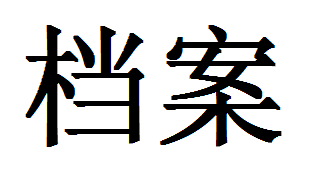
\includegraphics[width=\textwidth]{dangan_origin}
  \end{minipage}
  }
  \subfloat[]{
  \label{pic:dangan_dilated}
  \begin{minipage}[t]{0.3\textwidth}
    \centering
    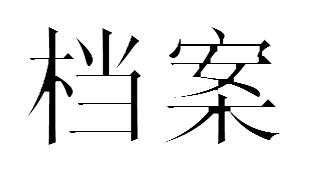
\includegraphics[width=\textwidth]{dangan_dilated}
  \end{minipage}
  }
  \subfloat[]{
  \label{pic:dangan_eroded}
  \begin{minipage}[t]{0.3\textwidth}
    \centering
    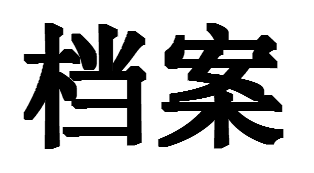
\includegraphics[width=\textwidth]{dangan_eroded}
  \end{minipage}
  }
  \caption{图片的膨胀和腐蚀}
  \label{pic:dangan}
\end{figure}

对图片的灰度化、二值化、膨胀和腐蚀操作有所了解以后,我们就可以利用这些图像处理方法,来进行图片分类任务了。前面我们提到我们是通过比较图片与三种版式图片的相似性来确定图片的版式,如

\section{预处理模块}     % 1000字
\subsection{方案选取}

\section{OCR模块}     % 6000字
\subsection{方案选取}

\section{字段解析模块}  %3000字
当含有文本的图片数据经过OCR模块以后,会被转换为文本,这些文本需要进行一定的加工,才能得到我们想要的各字段数据。总体来说,原始的文本需要经过数据清洗、字段匹配、目标文本提取等步骤。我们也可以认为这是数据的“后处理”过程。

\subsection{数据清洗}
数据清洗主要有两大功能,一是对文本的冗余信息(如因为图片噪声而产生的冗余符号)进行剔除,二是对文本进行简单的矫正。这两部分实现难度不大,却对之后的字段匹配过程有着很大的帮助。
\subsubsection{冗余信息剔除}
\subsubsection{文本矫正}

\subsection{字段匹配}
某段文本属于哪一个字段呢?这就需要对文本的具体内容进行理解划分了,例如若要判断
\subsubsection{StartsWith匹配}
\subsubsection{Includes匹配}


\section{数据存储模块} %500字
